\newprob{1718522323}
{
    % Active phys p361 q13
    一顆小行星正逼近地球。
    \begin{parts}
        \part 試證明小行星因地球引力產生的加速度與其 質量無關。 \zzh{2}
        \part 當小行星在地球表面上空10 000m,地球引 力對小行星產生的加速度為多少? \zzh{2}
        \part 小行星逼近地球時不斷獲得動能。
        \begin{subparts}
            \subpart 小行星在較高的高度水平時,獲得動能 的率較低還是較高?試扼要解釋。\zzh{2}
            \subpart 小行星所獲得的動能從何而來?\zzh{1}
        \end{subparts}
    \end{parts}
}{
    \par{\par\centering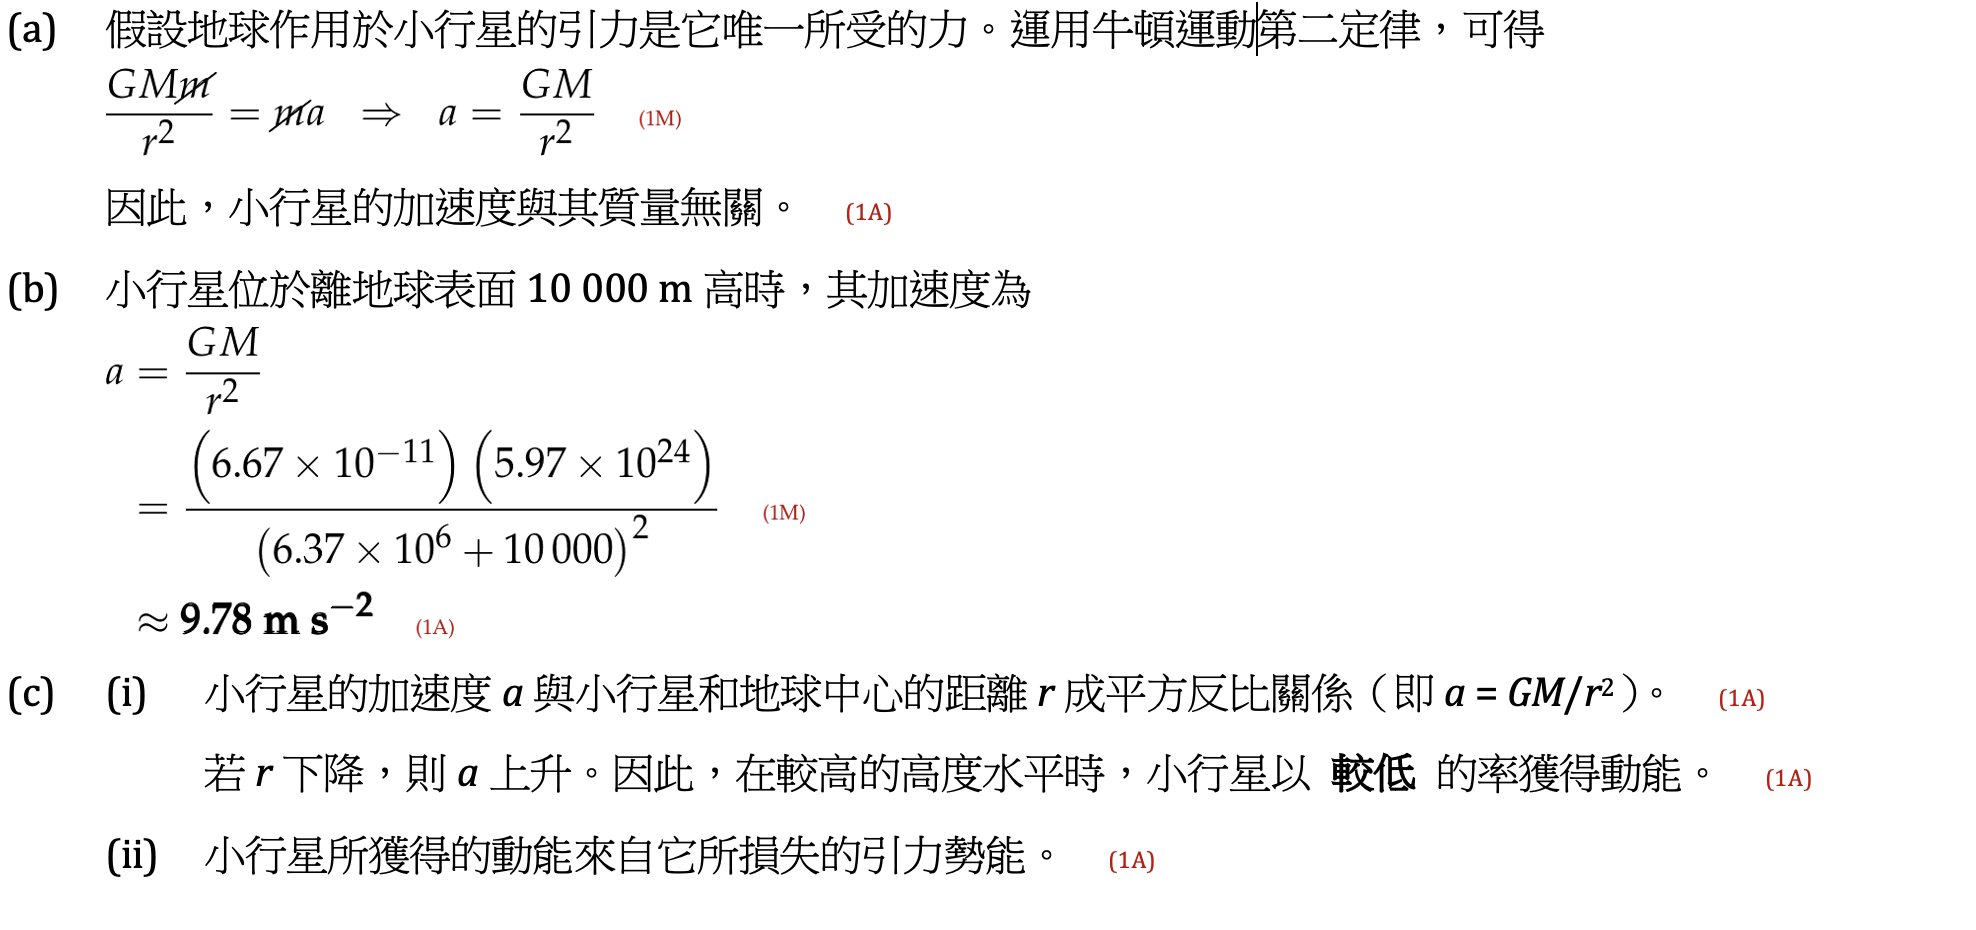
\includegraphics[width=\textwidth]{./img/ch_ACtransformer_lq_2024-06-17-15-51-44.png}\par}
}

\newprob{1718522327}
{
    一通訊衛星繞着地球以圓形軌道 運行,其週期為24小時。而這衛星保持在赤道上 空的某一位置。
    \par 已知:地球的半徑 $r_E= \qty{6400}{km}$
    \begin{parts}
        \part \begin{subparts}
            \subpart 求該通訊衛星的軌道半徑。\zzh{3}
            \subpart 求該通訊衛星的軌道速率。\zzh{2}

        \end{subparts}
        \part 下圖顯示於太空中的一點$X$,$O$為地球的中 心。
        \par{\par\centering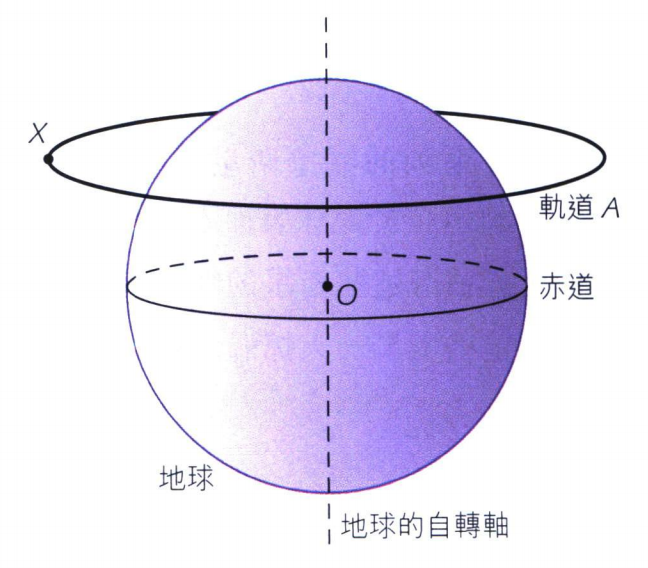
\includegraphics[width=.4\textwidth]{./img/ch_ACtransformer_lq_2024-06-16-15-26-59.png}\par}
        \begin{subparts}
            \subpart 一衛星位於X,在圖中繪出由地球作用 於該衛星的引力。\zzh{1}
            \subpart 試簡單解釋為甚麼若只受地球引力的影 響,該衛星不可能在圖中所示的圓形軌 道A 上運行。 \zzh{1}
        \end{subparts}
    \end{parts}
}{
    \par{\par\centering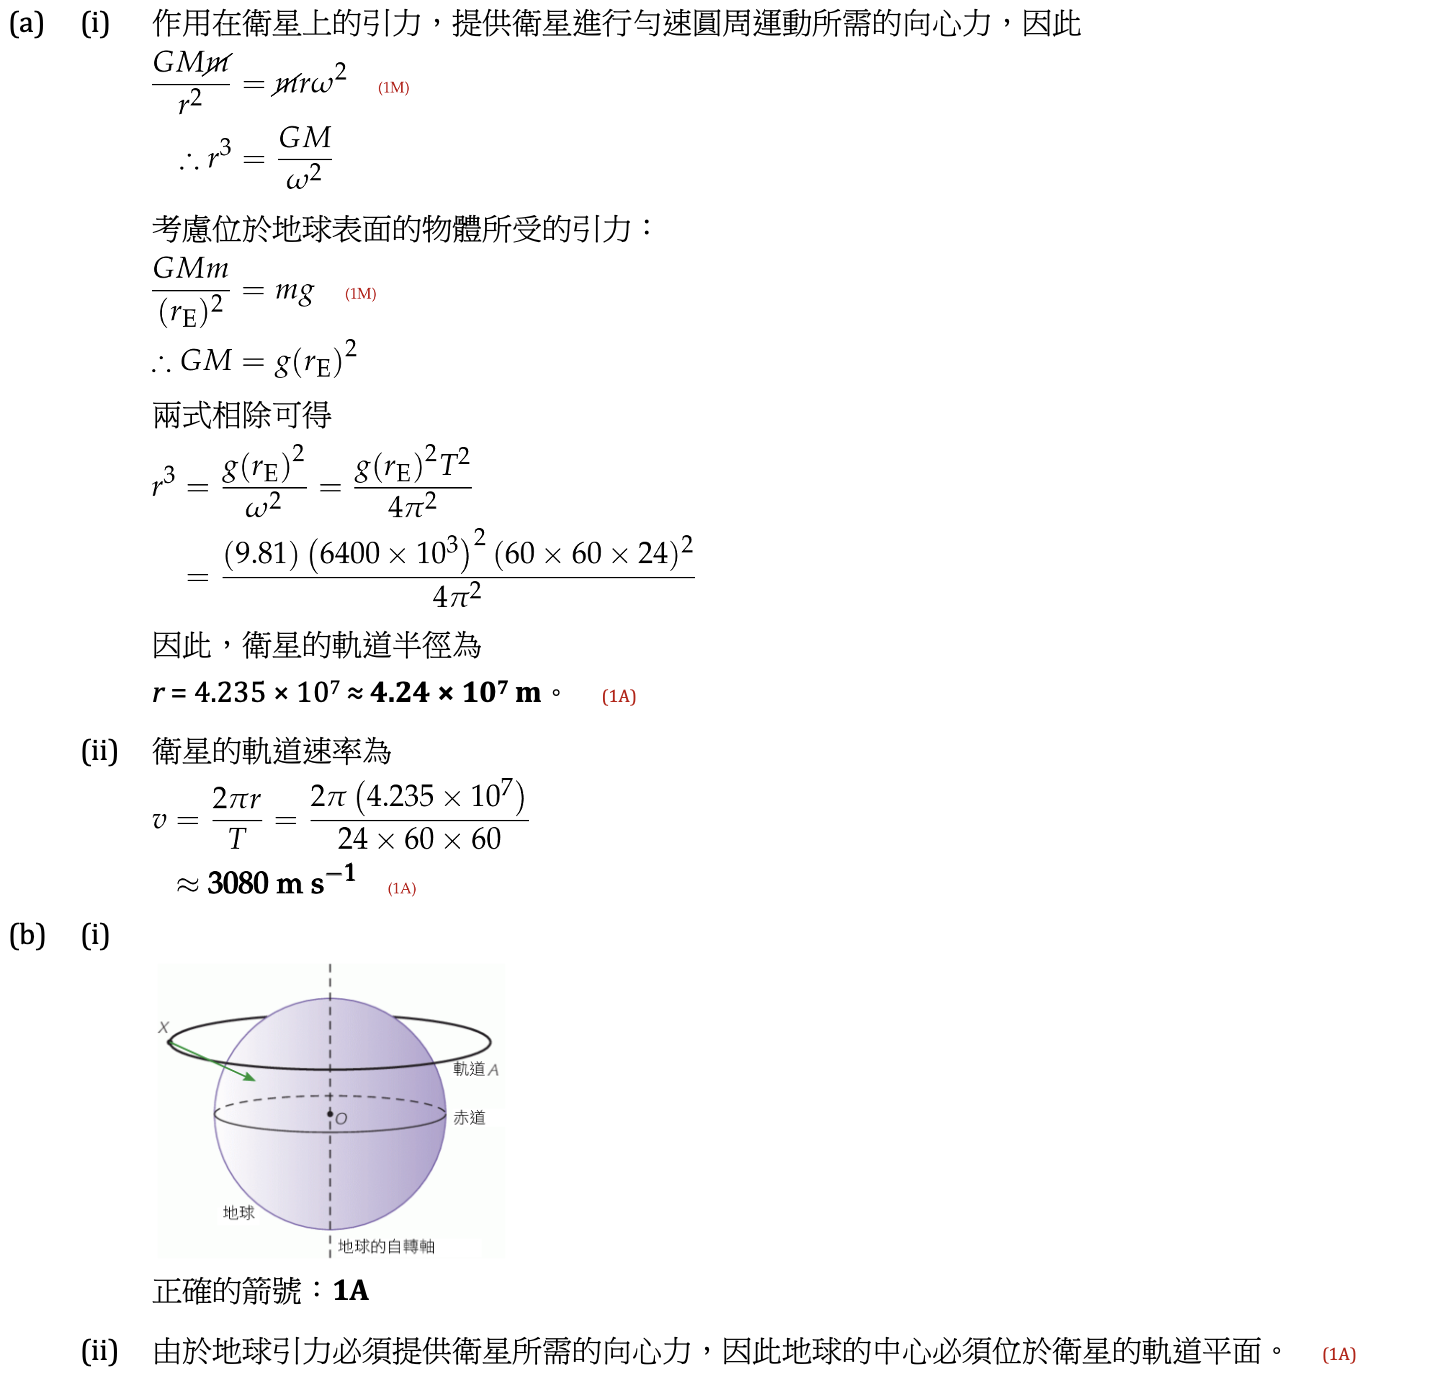
\includegraphics[width=\textwidth]{./img/ch_ACtransformer_lq_2024-06-17-15-52-38.png}\par}
}